\chapter{A brief introduction to Lie theory} \label{sec:Lie-theory}
In Chapter \ref{ch:3d-geometry} we saw that orientations and poses lie on manifolds in higher-dimensional spaces.
This makes it complicated to add increments, represent uncertainty and perform differentiation for such variables, since they do not have the same properties as vectors in vector spaces.

As an example, consider perturbing a rotation matrix $\matR \in \SO(3)$ by adding a matrix $\delta \matR \in \bbR^{3 \times 3}$.
This is problematic since for some $\delta \matR$ we have $\matR + \delta \matR \notin \SO(3)$, which means that the perturbation in general will not produce a new rotation matrix.
This also means that such perturbations is not a proper way to express the derivative of functions of rotation matrices.

We will in this chapter give a very brief introduction to a selection of extremely useful principles of \emph{Lie theory}.
The resulting mathematical framework will enable us to formulate estimation problems properly and with ease, by giving us the tools needed to work with rotations and poses \emph{on the manifold}.

Most of this chapter is heavily based on \cite{SolaARobotics}, as well as  \cite{Eade2013LieTransformations, barfoot2017state}.
It is meant as a practical introduction to the subject, and is not a proper introduction to the underlying theory as such.
Please see to the references above for more information.


\section{The Lie group}
\begin{figure}[htb]
    \centering
    \adjincludegraphics[width=0.5\columnwidth, trim={0 0 {.45\width} 0}, clip]{figures/manifold_tg.pdf}
    \caption{A manifold $\cM$ with the tangent vector space $\cT\cM_\cX$ at the point $\cX$. 
    In Lie groups, the manifold looks the same at every point, and all tangent spaces at any point are therefore alike.\\
    (Image source: \cite{SolaARobotics}; Cropped; licensed under \href{https://creativecommons.org/licenses/by-nc-sa/4.0/}{CC BY-NC-SA 4.0})}
    \label{fig:smooth-manifold}
\end{figure}
%
Informally, a Lie group is both a smooth differentiable manifold and a group satisfying the group axioms.
A group $(\cG, \circ)$ is a set $\cG$ with a composition operation $\circ$ that satisfies the axioms
\begin{align}
  \text{Closure under $\circ$} \; &: \quad \cX \circ \cY \in \cG\\
  \text{Identity $\cE$} \; &: \quad \cE \circ \cX = \cX \circ \cE = \cX \label{eq:lie-identity}\\
  \text{Inverse $\cX^{-1}$} \; &: \quad \cX^{-1} \circ \cX = \cX \circ \cX^{-1} = \cE\\
  \text{Associativity} \; &: \quad (\cX \circ \cY) \circ \cZ = \cX \circ (\cY \circ \cZ)
\end{align}
for elements $\cX, \cY, \cZ \in \cG$.

Lie groups can also transform elements of other sets.
Given a Lie group $\cM$ and a set $\cV$, we denote by $\cX \cdot v$ the \emph{action} of $\cX \in \cM$ on $v \in \cV$.
A group action must satisfy the axioms
\begin{align}
  \text{Identity} \; &: \quad \cE \cdot v = v\\
  \text{Compatibility} \; &: \quad (\cX \circ \cY) \cdot v = \cX \cdot (\cY \cdot v).
\end{align}

Since Lie groups are smooth manifolds, the group operations and actions are smooth, and look like operations on a vector space locally.
In fact, there is a unique tangent space at each point on the manifold that captures the local structure of the group (Figure~\ref{fig:smooth-manifold}).
This tangent space is a vector space that allows linear algebra and calculus.

In Lie groups, the local properties of smooth manifolds, which lets us do calculus, are combined with the global properties of groups, which lets us perform nonlinear composition and transformations on different objects.
We will in this chapter see how we can exploit these properties to perform perturbations and handle uncertainty on any element of the Lie group manifolds.
In Chapter~\ref{ch:jacobians} we will build upon this to define and compute derivatives on the manifolds. 

The orientation group $\SO(3)$ and pose group $\SE(3)$ introduced in chapter~\ref{ch:3d-geometry} are both examples of \emph{matrix Lie groups}.
These are Lie groups where the elements of the group are matrices, the composition operation is matrix multiplication, and the inversion operation is matrix inversion.
The action on vectors is $\matR \cdot \vecx \triangleq \matR \vecx$ for rotations $\matR \in \SO(3)$ and $\matT \cdot \vecx \triangleq \matR \vecx + \vect$ for poses $\matT \in \SE(3)$.
The group of vectors under addition $(\bbR^n, +)$ is actually also an example of a Lie group.
We will continue with a general introduction to Lie theory, which will cover all of these groups and more.
The properties of specific groups are summarised in appendix \ref{ch:useful-lie-groups}.


\section{The Lie algebra}
\begin{figure}[htb]
    \centering
    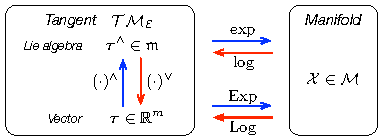
\includegraphics[width=0.8\columnwidth]{figures/maps.pdf}
    \caption{Mappings between the manifold $\cM$ and the representations of its tangent space at the identity $\cT \cM_\cE$.
    The hat $(\cdot)^\wedge$ and vee $(\cdot)^\vee$ operators map to/from the Lie algebra $\fm$ and tangent vector space $\bbR^m$. $\exp(\cdot)$ and $\log(\cdot)$ map the Lie algebra to/from the manifold, and $\Exp(\cdot)$ and $\Log(\cdot)$ are shortcuts to map the tangent vector space directly to/from $\cM$.\\
    (Image source: \cite{SolaARobotics}; licensed under \href{https://creativecommons.org/licenses/by-nc-sa/4.0/}{CC BY-NC-SA 4.0})}
    \label{fig:lie-maps}
\end{figure}
The structure of the tangent spaces on a Lie group manifold $\cM$ is the same everywhere.
We will denote the tangent space to $\cM$ at $\cX$ as $\cT \cM_\cX$, as illustrated in Figure~\ref{fig:smooth-manifold}.
The tangent space at the identity $\cT \cM_\cE$ is called the \emph{Lie algebra} of $\cM$, and is denoted $\fm$:
\begin{equation}
  \text{Lie algebra} \; : \quad \fm \triangleq \cT \cM_\cE.
\end{equation}

The Lie algebra $\fm$ is a vector space, and although its elements $\vectau^\wedge \in \fm$ can have non-trivial structures, they can be \emph{identified} with vectors $\vectau \in \bbR^m$, where $m$ is the dimensionality of $\cM$.
This is done by expressing $\vectau^\wedge$ as a linear combination of some base elements $\matE_i$, where $\matE_i$ are called the \emph{generators} of $\fm$.
We may in this way map between $\bbR^m$ to $\fm$ and vice versa with two mutually inverse linear maps called \emph{hat} and \emph{vee}:
\begin{align}
  \text{Hat:} \;& (\cdot)^\wedge : \bbR^m \to \fm ; \quad\quad \vectau^\wedge = \sum_{i = 1}^m \tau_i \matE_i\\
  \text{Vee:} \;& (\cdot)^\vee : \fm \to \bbR^m ; \quad\quad \vectau = (\vectau^\wedge)^\vee = \sum_{i = 1}^m \tau_i \vece_i,
\end{align}
where $\vece_i$ are the basis vectors of $\bbR^m$ so that $\vece^\wedge_i = \matE_i$ (Figure~\ref{fig:lie-maps}).
This lets us represent elements in the Lie algebra using vectors in a Cartesian vector space, which may be manipulated with linear algebra using matrix operations.


\section{The exponential map}
\begin{figure}[htb]
    \centering
    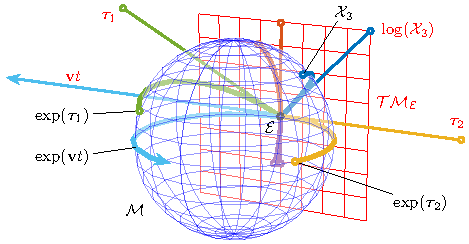
\includegraphics[width=0.9\columnwidth]{figures/exponential.pdf}
    \caption{An illustration of the relation between the Lie group and the Lie algebra.
    The Lie algebra $\cT\cM_\cE$ is the tangent space to the Lie group's manifold $\cM$ at the identity $\cE$.
    The exponential map wraps straight paths through the origin on the Lie algebra over the manifold along the corresponding geodesic.
    The logarithmic map unwraps curved and nonlinear paths on the manifold onto the linear Lie algebra.
    All points on the manifold has an exact equivalent on the tangent space.\\
    (Image source: \cite{SolaARobotics}; licensed under \href{https://creativecommons.org/licenses/by-nc-sa/4.0/}{CC BY-NC-SA 4.0})}
    \label{fig:lie-exponential}
\end{figure}
%
The \emph{exponential map} transfers elements of the Lie algebra $\vectau^\wedge \in \fm$ to elements of the group $\cX \in \cM$:
\begin{equation}
  \exp: \fm \to \cM; \quad\quad \cX = \exp(\vectau^\wedge).
\end{equation}
Intuitively, it wraps the tangent element over the manifold following the \emph{geodesic}, which in some sense is the shortest route along the manifold (Figure~\ref{fig:lie-exponential}).
The exponential map is \emph{exact} for all tangent elements, but does not always have a closed form expression.

The inverse transformation is the \emph{logarithmic map},
\begin{equation}
  \log: \cM \to \fm; \quad\quad \vectau^\wedge = \log(\cX),
\end{equation}
which unwraps elements on the manifold onto the tangent space (Figure~\ref{fig:lie-exponential}).

The \emph{capitalised exponential and logarithmic maps} are convenient compositions that lets us map vector elements $\vectau \in \bbR^m$ directly to group elements $\cX \in \cM$, and vice versa.
These are given by
\begin{alignat}{3}
  &\Exp: \bbR^m \to \cM; \quad\quad \cX &&= \Exp(\vectau) &&\triangleq \exp(\vectau^\wedge)\\
  &\Log: \cM \to \bbR^m; \quad\quad \vectau &&= \Log(\cX) &&\triangleq \log(\cX)^\vee.
\end{alignat}

Figure~\ref{fig:lie-maps} gives an overview of the different operators we can use to map between the manifold $\cM$ and the representations of its tangent space at the identity $\cT\cM_\cE$.
Additional properties of the exponential map is given in \cite{SolaARobotics, barfoot2017state}.

\section{Right and left perturbations} \label{sec:lie-right-left-perturbations}
The exponential map allows us to perform perturbations on elements $\cX$ on the manifold expressed as tangent space vectors $\vectau$ by combining one $\Exp$/$\Log$ operation with one composition.
Since the composition is non-commutative, the order of the operands is important for how the perturbations are performed.

With the combination
\begin{equation}
  \cX \circ \Exp(\prescript{\cX}{}{\vectau}),
\end{equation}
the perturbation is on the right side of the composition.
The tangent space vector $\prescript{\cX}{}{\vectau}$ therefore belongs to the tangent space at $\cX$, as denoted by the left superscript.
Following the convention we have used in Chapter~\ref{ch:3d-geometry}, we say that $\prescript{\cX}{}{\vectau}$ is expressed in the \emph{local} frame at $\cX$.

When we perform the perturbation on the left
\begin{equation}
 \Exp(\prescript{\cE}{}{\vectau}) \circ \cX,
\end{equation}
we have $\prescript{\cE}{}{\vectau} \in \cT\cM_\cE$, and we say that $\prescript{\cE}{}{\vectau}$ is expressed in the \emph{global} frame.

\begin{example}[frametitle=Local and global perturbations on poses] \label{ex:local-global-pert}
{
  \centering
  \adjincludegraphics[width=0.9\columnwidth, trim={{.1\width} {.25\height} {.15\width} {.15\height}}, clip]{figures/perturbation_illustration.pdf}
  \captionsetup{type=figure}
  \captionof{figure}{A world frame $\cF_w$ and a camera frame $\cF_c$. 
  A perturbation along the $x$-axis is performed on the right- and left-hand sides of the pose $\matT_{wc}$. 
  This corresponds to perturbations locally in the camera frame, and globally in the world frame, respectively.}
  \label{fig:perturbation-example}
  \par
}
The pose of a camera relative to the world frame is expressed as $\matT_{wc}$.
Perturbations on the right side of $\matT_{wc}$ are performed in the local camera coordinate frame, \emph{before} the transformation between the coordinate frames.
Perturbations on the left side are performed in the global world coordinate frame, \emph{after} the transformation.

The tangent vector $\vecxi = \begin{bmatrix}2 & 0 & 0 & 0 & 0 & 0\end{bmatrix}\trans$ corresponds to an increment of 2 units in the $x$-direction (see Section~\ref{sec:SE3_group}).
Figure~\ref{fig:perturbation-example} shows the result of perturbing $\matT_{wc}$ with $\vecxi$ locally along the $x$-axis of $\cF_c$ with $\matT_{wc}\Exp(\vecxi)$, and globally along the $x$-axis of $\cF_w$ with $\Exp(\vecxi)\matT_{wc}$.
\end{example}

We will in the following mostly consider local right side perturbations, although the left side convention is also common.
See \cite{SolaARobotics, barfoot2017state} for corresponding discussions covering left perturbations.


\section{Plus and minus operators} \label{sec:lie-plus-and-minus}
It is convenient to express right perturbations using the right plus and minus operators
\begin{alignat}{3}
  \cY &= \cX \oplus \prescript{\cX}{}{\vectau} &&\triangleq \cX \circ \Exp(\prescript{\cX}{}{\vectau}) &&\in \cM \label{eq:lie-plus-def}\\
  \prescript{\cX}{}{\vectau} &= \cY \ominus \cX &&\triangleq \Log(\cX^{-1} \circ \cY) &&\in \cT\cM_\cX. \label{eq:lie-minus-def}
\end{alignat}
The plus operator lets us increment an element $\cX$ with a tangent space vector $\prescript{\cX}{}{\vectau}$, while the minus operator lets us compute the corresponding tangent space vector between the two elements $\cX$ and $\cY$.
We will later use these operators to define derivatives on the manifold (Section~\ref{sec:derivative-Lie}).

It is also possible to define left plus and minus operators
\begin{alignat}{3}
  \cY &= \prescript{\cE}{}{\vectau} \oplus \cX &&\triangleq \Exp(\prescript{\cE}{}{\vectau}) \circ \cX &&\in \cM\\
  \prescript{\cE}{}{\vectau} &= \cY \ominus \cX &&\triangleq \Log(\cY \circ \cX^{-1}) &&\in \cT\cM_\cE.
\end{alignat}
Notice that while left and right $\oplus$ are distinguished by the operands, $\ominus$ is ambiguous.
Since we mostly consider right perturbations, we will also use the right definitions of $\oplus$ and $\ominus$ as default.

\begin{example}[frametitle=Interpolation on the manifold]
We can interpolate between two vectors $\vecx_1$ and $\vecx_2$ with the linear interpolation scheme
\begin{equation} \label{eq:vec-interp-example}
  \vecx = (1-\alpha) \vecx_1 + \alpha \vecx_2, \quad \alpha \in [0,1].
\end{equation}
This scheme will not work in general for Lie groups, since not all Lie groups are closed under addition.
For poses $\matT_1, \matT_2 \in \SE(3)$ for example, we will get
\begin{equation}
  (1-\alpha) \matT_1 + \alpha \matT_2 \notin \SE(3)
\end{equation}
for some values of $\alpha \in [0,1]$.

We can instead define a proper interpolation scheme on the manifold using Lie algebra.
The tangent vector between $\cX_1$ and $\cX_2$ in $\cT\cM_{\cX_1}$ is given by $\cX_2 \ominus \cX_1$.
The interpolation scheme
\begin{subequations}
\begin{align}
  \cX &= \cX_1 \oplus \alpha(\cX_2 \ominus \cX_1)\\
  &= \cX_1 \circ \Exp(\alpha \Log(\cX_1^{-1} \circ \cX_2))
\end{align}
\end{subequations}
will therefore move steadily along the geodesic from $\cX_1$ to $\cX_2$.

{
  \centering
  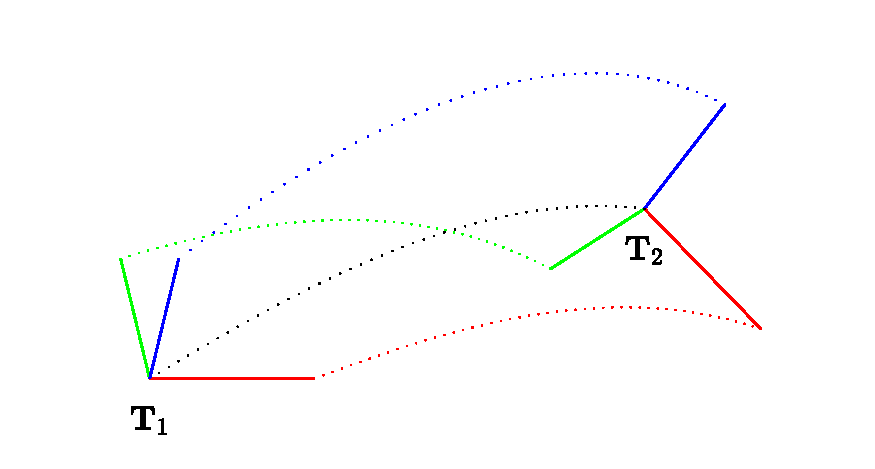
\includegraphics[width=0.75\columnwidth]{figures/pose_interpolation.pdf}
  \captionsetup{type=figure}
  \captionof{figure}{Interpolation along the manifold between two poses $\matT_1$ and $\matT_2$.}
  \label{fig:pose-interpolation}
  \par
}
For poses $\matT_1, \matT_2 \in \SE(3)$, we get
\begin{subequations}
\begin{align}
  \matT &= \matT_1 \circ \Exp(\alpha \Log(\matT_1^{-1} \circ \matT_2))\\
  &= \matT_1(\matT_1^{-1} \matT_2)^\alpha. \label{eq:pose-interp-example-exp}
\end{align}
\end{subequations}
An example of the interpolated motion along the manifold between two poses is shown in Figure~\ref{fig:pose-interpolation}.
We see that it follows a screw motion, corresponding to constant angular velocity, and constant translational velocity locally, so that the direction is constantly changed in the global frame.

{
  \centering
  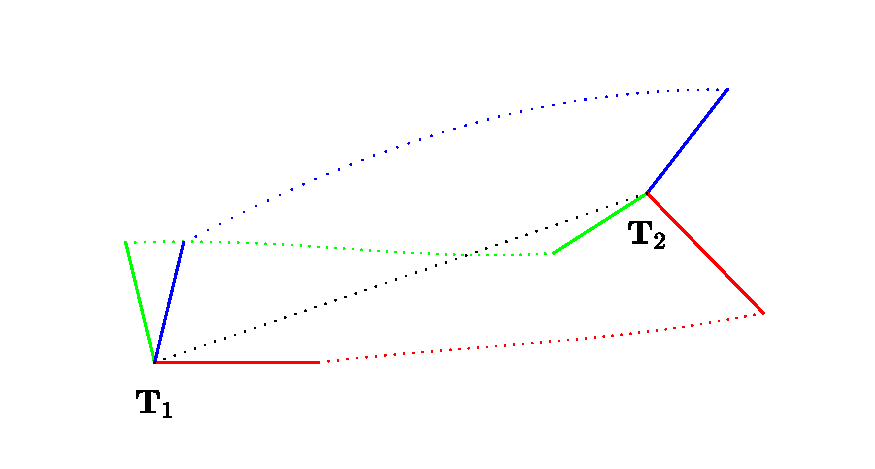
\includegraphics[width=0.75\columnwidth]{figures/pose_interpolation_hybrid.pdf}
  \captionsetup{type=figure}
  \captionof{figure}{Separate interpolation of rotation and position between two poses $\matT_1$ and $\matT_2$.}
  \label{fig:pose-interpolation-hybrid}
  \par
}
An alternative is to interpolate orientation and position separately (see the hybrid representation in Section~\ref{sec:hybrid-representation}).
For the poses $\matT_1 = \begin{bsmallmatrix} \matR_1 & \vect_1\\ \matr{0}\trans & 1 \end{bsmallmatrix}$ and $\matT_2 = \begin{bsmallmatrix} \matR_2 & \vect_2\\ \matr{0}\trans & 1 \end{bsmallmatrix}$, we get the separated interpolation scheme
\begin{align}
  \matR &= \matR_1 \oplus \alpha(\matR_2 \ominus \matR_1)\label{eq:rot-interp-example}\\ 
  \vect &= \vect_1 + \alpha(\vect_2 - \vect_1),
\end{align}
where the interpolated pose is given by $\matT = \begin{bsmallmatrix} \matR & \vect\\ \matr{0}\trans & 1 \end{bsmallmatrix}$, and we have rearranged \eqref{eq:vec-interp-example} a bit to show how similar the vector space and manifold schemes are.
Similarly to \eqref{eq:pose-interp-example-exp}, \eqref{eq:rot-interp-example} can also be expressed as $\matR = \matR_1(\matR_1\trans \matR_2)^\alpha$.
This separated scheme results in the linear translation motion shown in Figure~\ref{fig:pose-interpolation-hybrid}.
\end{example}

\section{The adjoint}
\begin{figure}[htb]
    \centering
    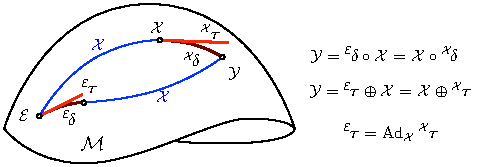
\includegraphics[width=0.75\columnwidth]{figures/adjoint.pdf}
    \caption{Two compositions $\cX \circ \prescript{\cX}{}{\delta}$ and $\prescript{\cE}{}{\delta} \circ \cX $ join the identity $\cE$ with the element $\cY$.
    Due to non-commutativity, the elements $\prescript{\cX}{}{\delta}$ and $\prescript{\cE}{}{\delta}$ are not equal.
    The corresponding tangent space vectors $\prescript{\cX}{}{\vectau} = \Log(\prescript{\cX}{}{\delta})$ and $\prescript{\cE}{}{\vectau} = \Log(\prescript{\cE}{}{\delta})$ are related by $\prescript{\cE}{}{\vectau} = \mAd_\cX \prescript{\cX}{}{\vectau}$, where $\mAd_\cX$ is the adjoint matrix of $\cM$ at $\cX$.\\
    (Image source: \cite{SolaARobotics}; licensed under \href{https://creativecommons.org/licenses/by-nc-sa/4.0/}{CC BY-NC-SA 4.0})}
    \label{fig:adjoint}
\end{figure}
%
In Section~\ref{sec:lie-right-left-perturbations} we saw that there are two natural ways of perturbing an element $\cX$ on the manifold by a tangent vector.
We can either right-perturb by a vector of the local tangent space, $\cX \circ \Exp(\prescript{\cX}{}{\vectau})$, or we can left-perturb by a vector of the tangent space at the identity, $\Exp(\prescript{\cE}{}{\vectau}) \circ \cX$.
One can show that this duality induces a relationship between the two tangent spaces called the \emph{adjoint of $\cM$ at $\cX$}, denoted by $\Ad_\cX$.

The \emph{adjoint action} of a group on its own Lie algebra is defined as
\begin{equation} \label{eq:adjoint}
  \Ad_\cX: \fm \to \fm; \quad\quad \Ad_\cX(\vectau^\wedge) \triangleq \cX \vectau^\wedge \cX^{-1}.
\end{equation}
As illustrated in Figure~\ref{fig:adjoint}, the adjoint determines a relation between the local and global tangent elements
\begin{equation}
  \prescript{\cE}{}{\vectau}^\wedge = \Ad_\cX(\prescript{\cX}{}{\vectau}^\wedge),
\end{equation}
so that 
\begin{equation}
  \prescript{\cE}{}{\vectau}^\wedge \oplus \cX = \cX \oplus \prescript{\cX}{}{\vectau}^\wedge.
\end{equation}

$\Ad_\cX()$ is a linear transformation, so we can define an equivalent matrix operator that maps the tangent vectors directly:
\begin{equation}
  \mAd_\cX: \bbR^m \to \bbR^m; \quad\quad \prescript{\cE}{}{\vectau} = \mAd_\cX \prescript{\cX}{}{\vectau}.
\end{equation}
The matrix $\mAd_\cX$ is called the \emph{adjoint matrix}, and it lets us linearly transform vectors of the tangent space at $\cX$ onto vectors of the tangent space at the identity $\cE$, corresponding to the same perturbation of $\cX$.
The adjoint matrix can be computed by applying the vee operator to \eqref{eq:adjoint}, so that
\begin{equation} \label{eq:adjoint-matrix}
  \mAd_\cX \triangleq (\cX \vectau^\wedge \cX^{-1})^\vee.
\end{equation}
See Appendix~\ref{ch:useful-lie-groups} for concrete examples.

Two useful properties of the adjoint matrix are
\begin{align}
    \mAd_{\cX^{-1}} &= \mAd_{\cX}^{-1}\\
    \mAd_{\cX \cY} &= \mAd_{\cX} \mAd_{\cY}.
\end{align}
It is typically cheaper to compute the left parts of these equalities.

We can use the adjoint matrix to manipulate the reference frame of the tangent space vectors in compositions and perturbations.
We can for example transform the from the local frame $j$ to the global frame $i$ with
\begin{align}
    \cX_{ij} \circ \Exp(\prescript{j}{}{\vectau})
    &= \Exp(\mAd_{\cX_{ij}} \prescript{j}{}{\vectau}) \circ \cX_{ij}\\
    &= \Exp(\prescript{i}{}{\vectau}) \circ \cX_{ij},
\end{align}
and we can transform back from the global frame $i$ to the local frame $j$ with
\begin{align}
    \Exp(\prescript{i}{}{\vectau}) \circ \cX_{ij}
    &= \cX_{ij} \circ \Exp(\mAd_{\cX_{ij}^{-1}} \prescript{i}{}{\vectau})\\  
    &= \cX_{ij} \circ \Exp(\mAd_{\cX_{ji}} \prescript{i}{}{\vectau})\\ 
    &= \cX_{ij} \circ \Exp(\prescript{j}{}{\vectau}).
\end{align}

Additional properties of the adjoint matrix is given in \cite{SolaARobotics, barfoot2017state}.

\begin{example}[frametitle=Computing global from local and vice versa]
In Example~\ref{ex:local-global-pert} we experienced the difference between applying a perturbation $\vecxi = \begin{bmatrix}2 & 0 & 0 & 0 & 0 & 0\end{bmatrix}\trans$ to the pose $\matT_{wc}$ locally on the right, and globally on the left.
The results are shown in Figure~\ref{fig:perturbation-example}.
We can use the adjoint matrix for poses $\mAd_\matT$ (see Section~\ref{sec:SE3_group}) to compute the corresponding perturbations in the other frame.

When $\vecxi$ is applied locally on the right side, the corresponding global perturbation is given by
\begin{equation}
  \prescript{w}{}{\vecxi} =
  \mAd_{\matT_{wc}} \vecxi = 
  \begin{bmatrix} 0 & 2 & 0 & 0 & 0 & 0 \end{bmatrix}\trans,
\end{equation}
which is an increment of 2 units along the $y$-axis of $\cF_w$.

When $\vecxi$ is applied globally on the left side, we can use the inverse pose to compute the corresponding local perturbation by
\begin{equation}
  \prescript{c}{}{\vecxi} =
  \mAd_{\matT_{wc}^{-1}} \vecxi = 
  \begin{bmatrix} 0 & \sqrt{2} & -\sqrt{2} & 0 & 0 & 0 \end{bmatrix}\trans,
\end{equation}
which is an increment of $\sqrt{2}$ units along the $y$-axis of $\cF_c$ and $-\sqrt{2}$ units along the $z$-axis of $\cF_c$.

We can use the adjoint matrix to transform tangent space vectors between coordinate frames, in the same way that we use poses to transform points.
\end{example}

